\section{Node Architecture}
\label{sec:node-arch}	
\begin{figure}[b!]
	\centering
	\label{fig:node}	
		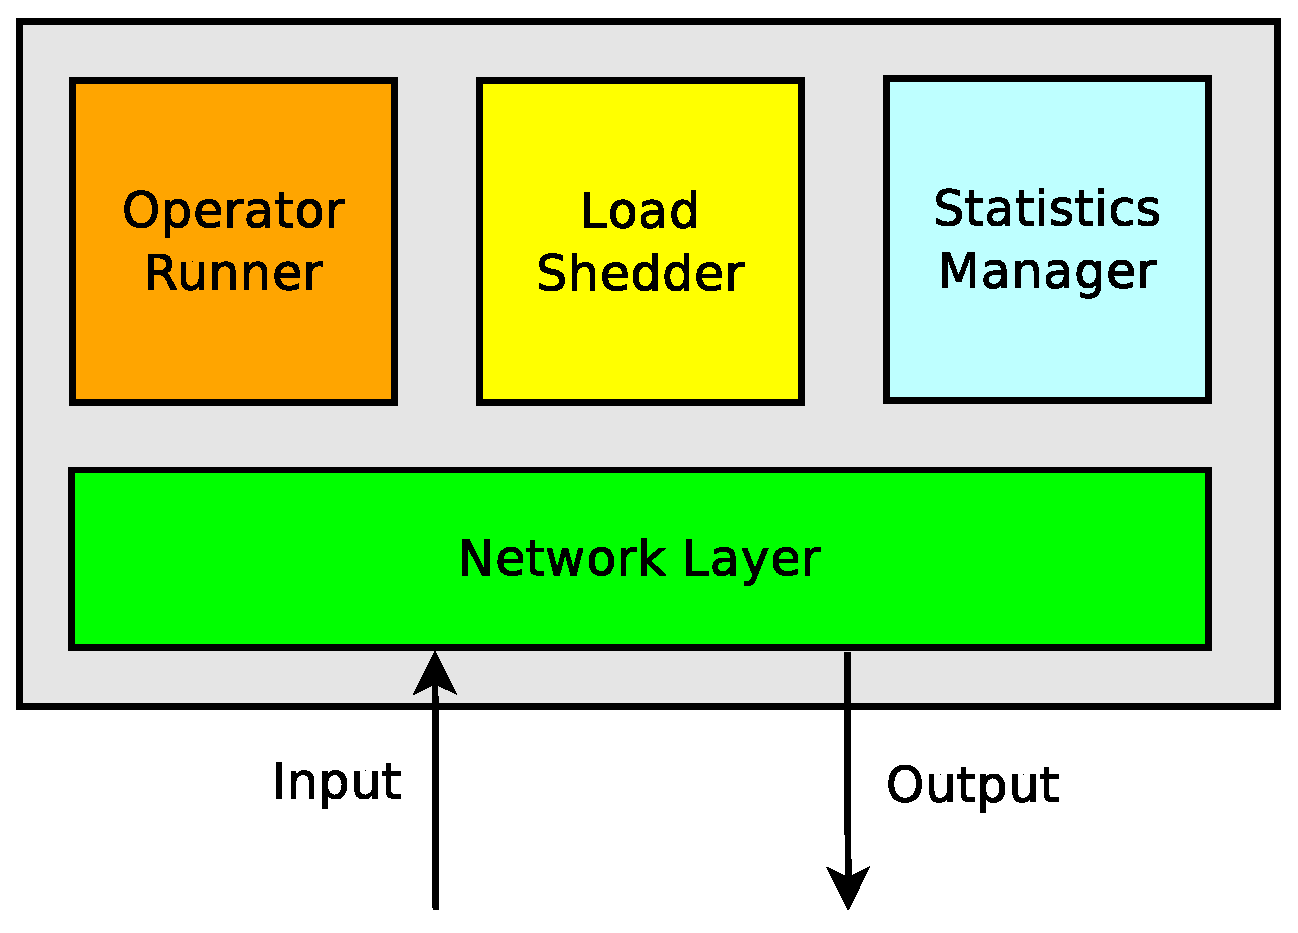
\includegraphics[width=0.5\textwidth]{img/tesi/node} 
		\caption{A high level view of a Processing Node, showing its internal logical components.}
\end{figure}
Every node in the system, at the core, is an instance of the DisspNode class, that gets specialised to
become either a processing node, a source, a submitter or an oracle. This section will describe the
internal structure of a DISSP \emph{processing node}. A system deployment comprises several processing
nodes, that can be hosted at many different sites, onto which queries can be deployed. Every node
usually hosts a portion of a query graph, called \emph{subquery}, while the complete query can span onto
several nodes. Every processing node can host several subqueries belonging to more than one query.

All inter-node communication passes through the \emph{Network Layer}, the component
responsible for the handling of \emph{command messages} and \emph{tuples}. When a command message is
received, it triggers an action that is performed directly at the network layer level. If a
\emph{batch of tuples} is received instead, it is passed directly the Operator Runner component. 
This layer also provides a \emph{web interface} that allows its remote monitoring.

The \emph{Operator Runner} is in charge of delivering the incoming tuples to the appropriate subqueries 
hosted at this node, and to execute the operators in their graphs employing a pool of concurrent threads
to achieve scalability.Once a subquery has completed its processing on a set of tuples, it sends them to
the network layer, that will send them to the following node to continue processing. 

If the incoming input is too large and the node resources are not sufficient to processes it completely
without running out of resources, the \emph{Load Shedder} component is in charge of selecting a portion
of it to be discarded in order to overcome the \emph{overload} condition. The selection of the tuples to
discard is determined by a \emph{shedding policy}, in particular this work focuses on a strategy trying
to \emph{fairly} shed tuples with the objective of maintaining a similar quality of processing, \sic value,
for all queries.
 
Finally, the last important component of each processing node is the \emph{Statistic Manager}, that is in
charge of collecting a number of statistics about the performance of the different queries and of the node as a whole. 

\subsection{Network Layer}  %2pp

The network layer is the component responsible for all the incoming and outgoing communications of a
processing node. It is composed of two threads: the \emph{NioConnector}, in charge of handling all
network communications, and the \emph{RequestHandler}, which interprets the content of the received messages and acts upon it.

The \emph{NioConnector} thread acts as a receiver for remote messages, as well as a sender for the
outgoing messages. All communication is done through TCP connections, this choice was made in order to preserve
the integrity of a network message. Using UDP would have increased the chances of a long message being
voided by the loss of one of its UDP chunks. The handling of sockets is based on the Java NIO library and
is completely asynchronous. This ensures a low communication overhead and allows one thread to deal with
all the I/O requests. This one-to-many design, where one thread is responsible for all sockets, was
preferred to the one-to-one approach, with one thread for each open socket, because of its simplicity and
efficiency, only employing one CPU core to handle network communication. Tests have shown that even under
heavy load and the presence of a large number of connections, the NioConnector never becomes a
performance bottleneck, since its semantic is only limited to the reading and writing of network data. 
As soon as an incoming message has been fully read, it is placed in a queue of pending messages, waiting
to be interpreted by the RequestHandler.

The \emph{RequestHandler} thread is responsible for the processing of incoming messages. It waits for the
NioConnector to place them into its queue and process them as soon as they become available. All inter
node communication within the system is encapsulated into \emph{messages}. 
The chosen format for messages is UTF-8 text, with
binary chunks expressed in Base64 encoding. This choice was made for simplicity and because it allows
for simpler debugging, even though a completely binary representation could have been used as a further
optimisation.
The initial task performed by the RequestHandler is to interpret the beginning of the message to
categorise it and process it accordingly. A message can be of 3 kinds. It can be a message containing
\emph{tuples} to be delivered to some subquery to be processed, it can contain a \emph{command
message} triggering the execution of a remote procedure call, or it can simply be the request to access
the \emph{web interface}.

\paragraph{Tuples handling.}
Once a message has been determined as containing a tuple payload, it is directly passed to the
\emph{Operator Runner} component, without further processing. The content of the message stays in network
format, thus being passed as a string. This follows the principle of \enmph{Lazy Deserialisation}, which
states that the conversion from network format of tuples should happen as late as possible. Tuple
objects are instantiated only when their are scheduled for processing, even their destination, the
queries they belong to, is not known until then.
 
The reason for this choice is that instantiating tuples and finding their destination is a costly process
and it could also be useless to perform it early, since at a later stage the whole batch could be dropped
by the \emph{Load Shedder}. Delaying this operation as much as possible ensures that no resources are
wasted to instantiate and route tuples that may never be processed. Tests have shown that an early
deserialisation also posed a great processing burden on the RequestHandler thread, which was not able to
handle all messages in a timely fashion under heavy load, leading to a growing message queue and
eventually raising an out-of-memory exception.

\paragraph{Command messages.}
A message can also contain a command, triggering the corresponding remote procedure call. This can be
used for communication purposes, reporting information about the status of a node or of a query to the
Oracle or the query Coordinator. Every node, for example, periodically reports its throughput, average
tuple latency and load information to the Oracle. Every node then also reports the achieved \sic value
for each query to the respective Coordinator, which in turns calculate an aggregated value to be sent to
the Oracle. 

Command messages can also be used to obtain information from another node or from the Oracle. For
instance, when a Coordinator is instantiating a query it sends a message to the Oracle requesting a list
of nodes onto which to deploy the query. During the initial connection stage, when the subqueries running
at different nodes need to connect to each other it is usual that a node has to wait a certain amount of
time for the other node to be ready to accept a connection. A message is used in this situation to probe
the availability of the another node and to wait until it becomes ready.

Another use for messages is to propagate certain values to a set of nodes. Every node, for example,
needs to be aware of the final \sic value achieved by all the queries that are running on it. Using the
global \sic value achieved by every query and comparing the local value of the tuples it processes the
Load Shedder can implement an intelligent dropping policy. So every Coordinator periodically spreads the
global \sic value of its query to all the nodes hosting its subqueries.

\paragraph{Web interface.}
The RequestHandler is also the gateway to the node web interface. When receiving a message it checks if
it is an HTTP request and if so it replies with a web page containing information about the current
status of the node, using the information obtained from the StatisticsManager. This includes the number
of subqueries hosted together with their performance, as well as some global metrics describing the
global status of the node, like its average throughput and latency.
When connecting to the Oracle, the web interface produces a report about the status of all processing
nodes, together with a summary of the performance achieved by all queries, sorted by \sic value. The web
interface of the Oracle is useful to monitor the overall performance of the system and to evaluate the
effectiveness of the shedding policy. 

\subsection{Operator runner.}

Once a batch of tuples has been received it gets passed to the Operator Runner to be processed. The
original message, still in its network format, is encapsulated into a \emph{work unit}, a Runnable class
representing a future job to be processed. This is submitted to a ThreadPoolExecutor and placed into a
pending queue, until one of the threads in the pool becomes available and executes it. The Work Unit
contains the logic to deserialise, route and process the tuples contained in the message it was
assigned. The last operator of the subquery graph usually is a Remote Sender, that takes the result of
the subquery computation and send it to the next processing node through the Network Layer. Once a Work
Unit has terminated its execution it terminates and frees its execution thread so that a new Work Unit
can be processed.

\paragraph{Thread pool.}
At the core of the \emph{Operator Runner} there is a \emph{thread pool}, ready to executes Work Units as
they are submitted. It is a subclass of ThreadPoolExecutor, that augments its parent class with the
possibility of stopping and resuming execution, needed by the Load Shedder to inspect the pending jobs
queue. The number of threads is set to the number of available CPU cores. The pending jobs queue is a
list of Work Unit. As soon as one of the threads in the pool is available it removes the oldest WorK Unit
from the queue and executes it. When the system is overloaded the number of items added to the queue is
larger than the number of items removed, thus making the size of the queue grow, and thus the latency of
processing, eventually leading to an out-of-memory exception. For this reason, the Thread Pool is
periodically interrupted by the Load Shedder, that inspects the pending batches and decides if there is
the need of dropping a certain portion of them in order to overcome overload. The choice about which ones
to discard is part of the shedding policy of the Load Shedder.

\paragraph{Work unit.}
A Work Unit is a container class implementing Runnable that contains the blueprint to deserialise, route
and process a batch of tuples. Once a Work Unit is removed from the pending jobs queue and selected
for processing, it gets executed by a thread from the pool. 
It starts by deserialising and instantiating the tuples contained in the message received
from the net. Then it checks to what query it should be delivered. In case the recipients are multiple,
it creates a copy of itself for each other query interested in its payload. Then it calls the
\texttt{.process()} method on the first operator of the query graph. This method takes the incoming
tuples ans executes the operator logic, producing one or more batches in output. The Work Unit passes
these tuples to the next operator and continues processing until it reaches the end of the local subquery
graph. A Work Unit will continue processing as long as possible, instead of creating a
new Work Unit for each operator, allowing the system to achieve a higher throughput by reducing overhead.
Not introducing a new Work Unit for each operator also guarantees that once a batch of tuples starts
processing it will not be touched by the load shedder, while the one Work Unit per operator approach
sometimes resulted in a batch being processed by a few operators just to be discarded by a later
execution of the load shedder. If the subquery graph contains an operator with more than one follower,
like in a fan-out query, the current Work Unit will continue processing on one branch, while creating a
new Work Unit for each other following operator. 

\subsection{Load Shedder}

The \emph{Load Shedder} is the component delegated to the \emph{overload} containment of a processing
node. When the amount of input tuples rises over a certain threshold the resources available at a node
become insufficient for their processing. These means that more tuples are given in input to a node than
the ones that it can process, thus leading to the accumulation of jobs in the pending queue. This leads
to a growing increase in latency for the tuples and to the never or the cost of processing ending growth
of the internal queues, until the available memory finishes, leading to a system crash. 

\paragraph{Periodic evaluation.}
The \emph{CheckOverload} thread periodically runs and evaluate the
current load situation of the node.
In the DISSP prototype a \emph{shedding interval} of 250ms has been chosen, which allows a timely response to
overcome an overload condition while keeping a reasonable performance overhead. Every time this thread
executes it calculates the number of tuples the node will be able to process before the next load check.
If this number is greater than the number of tuples currently in the queue waiting to be processed, the
system is not overloaded and there will be no dropping of tuples. On the other hand, if the number of
awaiting tuples is larger than the ones the node will manage to process, a certain amount needs to be
discarded. 

The system keeps track of its \emph{output rate}: the amount of tuples processed within one shedding
interval. It uses this to calculate the average time needed to process one tuple, called \emph{tuple
cost}.
Since the shedding interval is
fixed, it is possible to calculate the amount of tuples that the system will be able to process before
the new shedding iteration, by dividing the \emph{shedding interval} by the \emph{tuple cost}. These
provides the amount of tuples \emph{to keep}, subtracting this number from the \emph{total number of
tuples waiting}, the system obtains the \emph{amount of tuples to be dropped}.
These numbers depend on many factors, for example the number of tuples received by each subquery
hosted can be different in different interval, or the query semantic may produce a variable load
depending on the values contained in the incoming tuples (\ie in the presence of a Filter). Therefore the
system uses a \emph{sliding window} to average a value over a few past iteration, reducing the
variability of these variables.

\paragraph{Execution cycle.}
%The periodic cycle followed by the Load Shedder is as following:
Every time the Load Shedder thread executes it follows the same processing steps:
\begin{environment}
\singlespacing
\begin{enumerate}
  \item Pause the thread pool
  \item Calculate the amount of tuples to be shed
  \item Choose what tuples to shed
  \item Shed the chosen tuples
  \item Resume the thread pool
  \item Update the load metrics 
\end{enumerate}
\end{environment}
First, the thread pool has to be stopped, in order to count the number of tuple it contains in its
pending queue at this moment. The processing of tuples can not happen during the execution of the load
shedder, so that it can choose what tuples to drop from a static set. Then it estimates the amount of
tuples to be dropped, using the logic exposed in the previous paragraph.
 Once the number of tuples to keep is calculated the Load Shedder can make a decision about
what tuples should be dropped out of the ones available. This choice depends on the semantic of the Load
Shedder and is referred to as \emph{shedding policy}. A more detailed description of different shedding
policies will be given in Chapter~\ref{ch:shedding}. Then the actual tuples are dropped by
removing the corresponding Work Unit from the thread pool queue. In the DISSP
prototype the granularity of dropping is at the level of \emph{batches}, since this is the input/output
unit between operators and every Work Unit is associated with a batch. After performing the dropping of
tuples, the thread pool can be restarted and thus the processing of tuples. Before ending its cycle, the
Load Shedder calculates the new updates the current \emph{tuple cost} and other internal metrics. Once it
has finished executing, it calculates the time it took for processing, called \emph{shedding time}, it
subtracts it from its fixed interval of execution, called \emph{shedding interval}, obtaining the amount
of milliseconds to sleep before its next execution.

\subsection{Statistics Manager}

The \emph{Statistics Manager} is the component responsible for the calculation of the global performance
metrics of a processing node. It runs periodically, by default once a minute, and calculates a number of
statistics, some of which are logged locally and some propagated either to the Coordinator or to the
Oracle. The following is a list of the most significant metrics and their function:

\textbf{Average SIC:} The average \sic value achieved by queries hosted at this node. Every subquery is
aware of its global \sic value, as this value is propagated from the Coordinator to all the
participants nodes. This metric is sent to the Oracle and can be used during the deployment of
a new query. In the scope of a fair deployment strategy, a node already hosting pieces of queries
achieving a low global \sic value, should not be chosen as a host for a new subquery. Adding further load to the node
in fact may lead to an overload condition, thus further depleting the performance of the currently
running queries. 

\textbf{Average tuple drop:} The average number of tuples dropped by the node in a chosen time interval.
This value helps evaluating the amount of overload experienced by a node. This value is sent to the
Oracle and it can be used by a deploying strategy to place a new subquery onto nodes that are not
overloaded or to avoid placing it on a node experiencing already a high tuple loss. 

\textbf{Average Throughput:} The average number of tuples processed by the node in a chosen time
interval. This value can be used to evaluate the spare processing capacity of a node. By recording the
value of this metric when hitting an overload condition it is possible to have an indication about the
number of tuples per second that this node is able to process on average without any loss. This value is
sent to the Oracle and can help a deployment strategy to choose the least loaded nodes out of those
currently not experiencing overload.

\textbf{Average Latency:} The average latency in milliseconds for all the hosted subqueries. A measure of
how much time a tuple spends in this node, from when it is received to when it is delivered in output to
the next node. This value is sent to the Oracle and can be used to detect performance bottlenecks and to
evaluate the goodness of the chosen deployment strategy. A good strategy would result in similar
latencies at all nodes.

\textbf{Number of running subqueries:} a number used to check if the deployment strategy leads to an even
deployment or to a skewed distribution of the subqueries. This number is sent to the Oracle and can be
used to evaluate the goodness of the chosen deployment strategy.

\textbf{Number of connected subqueries:} a number used to check the correct deployment of a query.
Every subquery contains at least one incoming network operator (Remote Receiver) and one outgoing network
operator (Remote Sender). When the deployment is successful the number of established connection is equal
to the number of these operators, a discrepancy indicates that one or more queries are disconnected
either temporary or permanently. 


